% Title: gl2ps_renderer figure
% Creator: GL2PS 1.4.2, (C) 1999-2020 C. Geuzaine
% For: Octave
% CreationDate: Sat Sep 11 16:05:20 2021
\setlength{\unitlength}{1pt}
\begin{picture}(0,0)
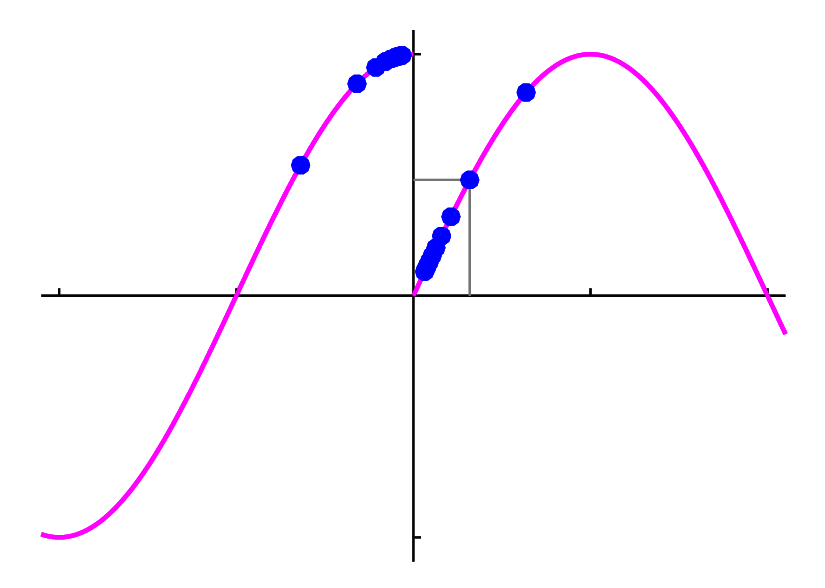
\includegraphics[width=7cm,height=5cm]{fig_teorema_funcao_continua}
\end{picture}%
\begin{picture}(198,141)(0,0)
\fontsize{10}{0}\selectfont\put(14.2074,62.6597){\makebox(0,0)[t]{\textcolor[rgb]{0.15,0.15,0.15}{{$-\pi$}}}}
\fontsize{10}{0}\selectfont\put(56.71,62.6597){\makebox(0,0)[t]{\textcolor[rgb]{0.15,0.15,0.15}{{$-\sfrac{   \pi}{2}$}}}}
\fontsize{10}{0}\selectfont\put(141.715,62.6597){\makebox(0,0)[t]{\textcolor[rgb]{0.15,0.15,0.15}{{$ \sfrac{   \pi}{2}$}}}}
\fontsize{10}{0}\selectfont\put(184.218,62.6597){\makebox(0,0)[t]{\textcolor[rgb]{0.15,0.15,0.15}{{$\pi$}}}}
\fontsize{10}{0}\selectfont\put(94.2243,12.1525){\makebox(0,0)[r]{\textcolor[rgb]{0.15,0.15,0.15}{{-1}}}}
\fontsize{10}{0}\selectfont\put(94.2243,128.115){\makebox(0,0)[r]{\textcolor[rgb]{0.15,0.15,0.15}{{1}}}}
\fontsize{10}{0}\selectfont\put(93.801,97.9316){\makebox(0,0)[r]{\textcolor[rgb]{0,0,0}{{$f(a_n)$}}}}
\fontsize{10}{0}\selectfont\put(112.742,64.3357){\makebox(0,0)[tl]{\textcolor[rgb]{0,0,0}{{$a_n$}}}}
\end{picture}
